% Section 4. Grounded rewrite 2026-11-03 (branch docs/cep-grounded-draft). Numbers: scripts/rerun_paper_numbers.py
% (rows 15-18, 21-23, 48-51; docs/optics/rerun_results.md); figures: python -m optics.plots, python -m optics.measure.
% Claim changes: papers/cep/CLAIM_CHANGES.md.
\section{Defocus structure and sharpness profile \emph{(RQ2)}}\label{sec:defocus}

\subsection{Circle of confusion}\label{sec:coc}

For a lens focused at $d_\mathrm{focus}$ with aperture diameter $f / N$, the geometric circle-of-confusion (CoC)
diameter at the sensor for an object at $d_o$ follows from similar triangles and Eq.~\eqref{eq:thinlens}
\citep{Pentland1987}:
\begin{equation}\label{eq:coc}
c(d_o) = K \, \frac{|d_o - d_\mathrm{focus}|}{d_o}, \qquad K = \frac{f^2}{N (d_\mathrm{focus} - f)}.
\end{equation}
The blur is asymmetric in $d_o$: it grows faster on the near side and saturates at $c_\infty = K = 38.12$~mm (F/1.6)
as $d_o \to \infty$. In the reciprocal variable $u = 1/d_o$ it is linear and symmetric about $u_\mathrm{focus}$,
\begin{equation}\label{eq:cocu}
c(u) = K \, d_\mathrm{focus} \, |u - u_\mathrm{focus}|,
\end{equation}
so a blur diameter alone does not tell whether an object lies in front of or behind the focused plane
\citep{SellentFavaro2014}; \secref{sec:sizing} addresses this ambiguity. Close to focus,
$c \approx K |\delta| / d_\mathrm{focus}$ with $\delta = d_o - d_\mathrm{focus}$.

\begin{figure*}
\centering
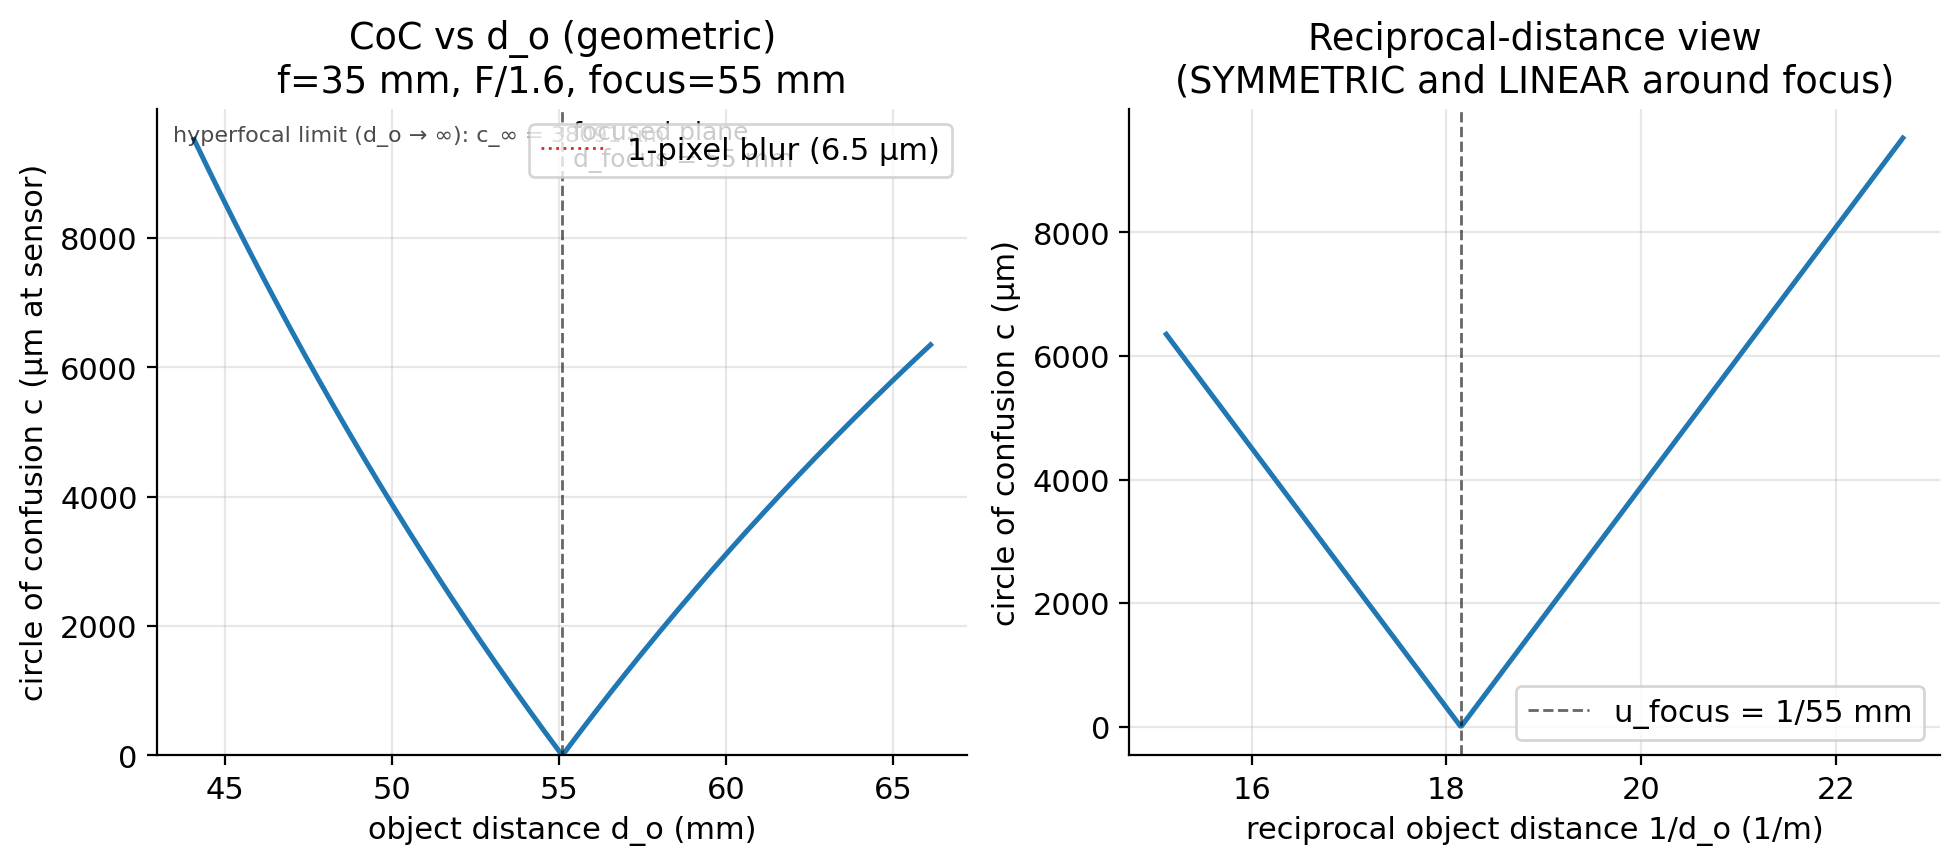
\includegraphics[width=0.85\textwidth]{02_coc_vs_distance}
\caption{\textbf{How does blur grow away from the focused plane?} Geometric CoC at F/1.6 against object distance
(left), asymmetric in $d_o$, and against reciprocal distance $u = 1/d_o$ (right), symmetric and linear about
$u_\mathrm{focus}$. The left CoC axis is logarithmic so that the dotted line of one geometric-mean PAL sample
(6.5~\um{} on the sensor) is visible; the legend gives the limit $c \to K$ for $d_o \to \infty$.}\label{fig:coc}
\end{figure*}

\subsection{Sharpness profile under a Gaussian PSF}\label{sec:psf}

We approximate the defocus point-spread function by a Gaussian whose width is proportional to the blur diameter,
$\sigma = k c$, where the constant $k$ depends on the camera \citep{Pentland1987,SubbaraoSurya1994}. We take
$k = 1/2$; a uniform disk of diameter $c$ would give $c/4$ per axis. The constant sets the width of the sharpness
peak, not its asymptotic exponent. The optical transfer function is then $|H(\nu)|^2 = \exp(-4 \pi^2 \sigma^2 \nu^2)$
at spatial frequency $\nu$. A Laplacian-type focus measure \citep{Pertuz2013} weights the image spectrum by $\nu^4$;
for a one-dimensional integral over a texture with a flat spectrum,
\begin{equation}\label{eq:sharpness}
S(\sigma) \propto \int_0^{\infty} e^{-4 \pi^2 (\sigma^2 + \sigma_0^2) \nu^2} \, \nu^4 \, \mathrm{d}\nu
\propto (\sigma^2 + \sigma_0^2)^{-5/2},
\end{equation}
where the floor $\sigma_0$ combines, in quadrature, half a geometric-mean PAL sample and the diffraction width
$\sigma_\mathrm{diff} \approx 0.42 \lambda N_w$, the Gaussian approximation of the paraxial Airy pattern
$\sigma \approx 0.21 \lambda / \mathrm{NA}$ with the image-side $\mathrm{NA} \approx 1/(2N_w)$
\citep{ZhangZerubia2007}. At macro magnification the working F-number is $N_w = N(1 + M)$, with the pupil
magnification taken as one; at $M = 1.743$ it is $2.74\,N$, and $\lambda = 550$~nm gives a diffraction FWHM at the
sensor of 2.4~\um{} (0.37 PAL samples) at F/1.6 (\code{scripts/rerun_paper_numbers.py}, rows 106--109). The exponent
$5$ is a property of these assumptions, not of the optics alone. The same integral taken in two dimensions over a
texture whose power spectrum falls as $|\nu|^{-\beta}$ gives $(\sigma^2 + \sigma_0^2)^{-(6 - \beta)/2}$. Composed with
Eq.~\eqref{eq:coc}, $S$ is a cusp in object distance: tall and narrow at the focused plane, with tails falling as
$|\delta|^{-5}$ once $\sigma \gg \sigma_0$, and not a Gaussian (\figref{fig:sharpness}).

\begin{figure*}
\centering
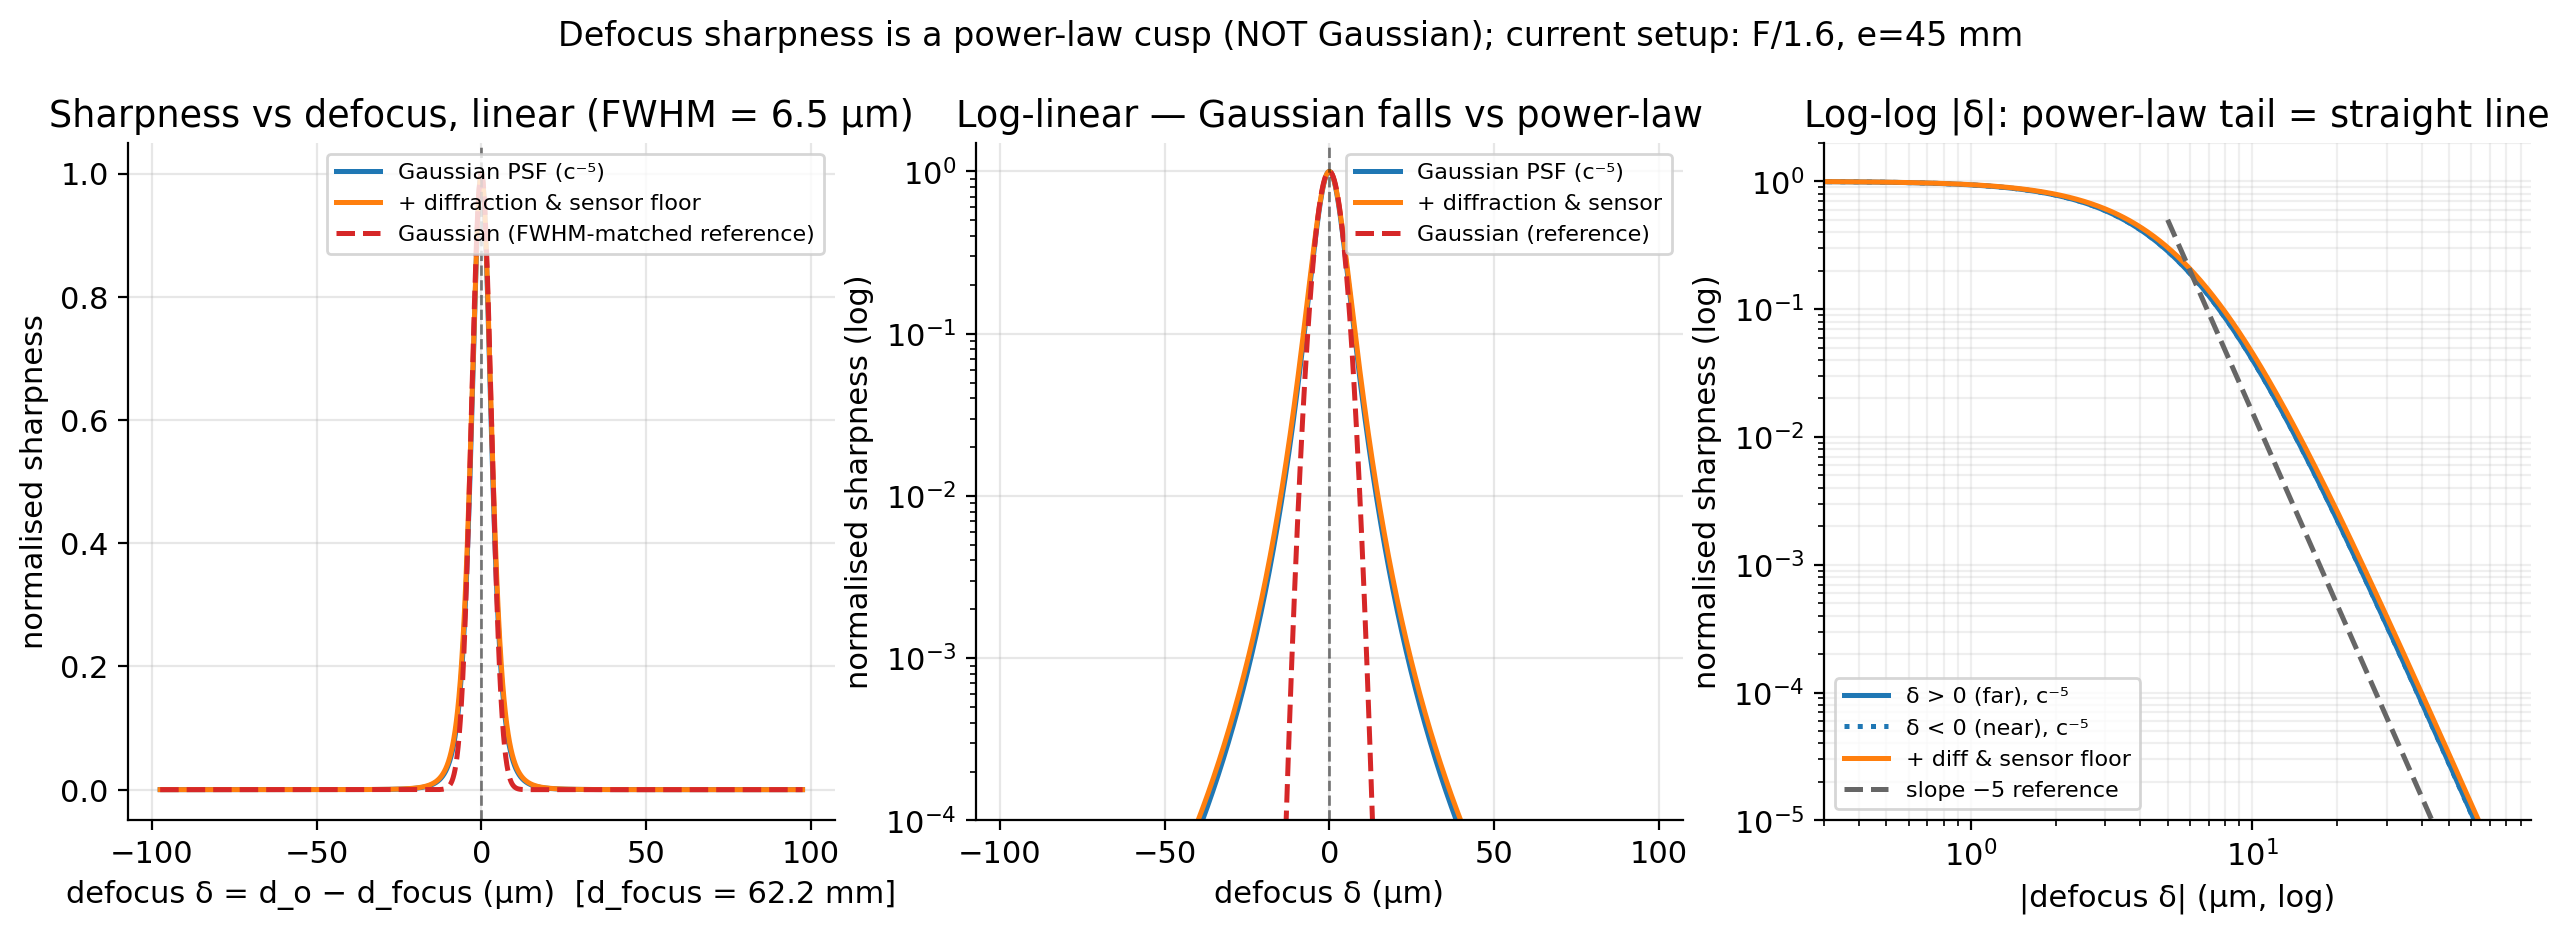
\includegraphics[width=0.82\textwidth]{03_sharpness_vs_distance}
\caption{\textbf{What shape does the model give the sharpness profile?} Modelled sharpness (Eq.~\ref{eq:sharpness})
against defocus $\delta = d_o - d_\mathrm{focus}$ at F/1.6, with the floor set by one PAL sample.
\textbf{Left} (linear): the peak has a full width at half maximum of 10.5~\um{} of object depth; a Gaussian of the
same FWHM is shown dashed. \textbf{Middle} (log $y$): the Gaussian falls off as a parabola, the model has heavy
tails. \textbf{Right} (log--log in $|\delta|$): the model tends to the slope of the $-5$ reference line as $|\delta|$
grows, which restates the model's asymptote and is not a measurement. The diffraction term changes the curve
only near $\delta = 0$.}\label{fig:sharpness}
\end{figure*}

\subsection{Depth of field}\label{sec:dof}

The in-focus slice is the depth range in which the CoC stays below one resolution element. For both recording types
that element is the PAL sample (\secref{sec:chain}), 6.53~\um{} on the sensor as a geometric mean; a 1080p clip
pixel (2.92~\um) is an upscaled fraction of a sample and does not resolve finer detail. \tabref{tab:dof} gives the
slice for both definitions, so that the effect of the choice is visible. With the PAL sample, the in-focus slice at
F/1.6 is $\pm 9.4$~\um. The geometric slice grows in proportion to $N$ (Eq.~\ref{eq:coc}; \figref{fig:dof}), but
diffraction grows with $N_w$: its FWHM reaches one PAL sample at about F/4.4 and is 1.8 samples at F/8 and 3.7
samples (23.9~\um) at F/16. Beyond about F/4 no depth meets the one-sample criterion, so the geometric $\pm 94$~\um{}
at F/16 bounds only the geometric blur and is not an in-focus slice. The iris is the only lever of the installed
hardware on the slice thickness, and diffraction caps it. Depths here are in air-equivalent thin-lens coordinates;
beyond the inner glass face, a paraxial depth in a medium of index $n_s$ is $n_s$ times longer.

The PAL sample as resolution element is an assumption, not a measurement, and it is optimistic. The analogue
bandwidth of camera and recorder is undocumented; even the BT.601 luma passband of 5.75~MHz \citep{ITUBT601}
resolves only about 600 points in the 52~\textmu s active line, against 720 samples; the two
interlaced fields of a moving slurry can halve the vertical resolution; and the H.264 compression of the recordings
removes fine texture. Each would coarsen the element and widen the slice in proportion. A measured edge-spread
function of the analogue chain would settle it \pending{effective resolution of the recorded PAL chain}.

\begin{table}
\centering\tabfont
\caption{In-focus half-slice (geometric CoC $\le$ one resolution element) and sharpness FWHM, in \textmu m of
air-equivalent object depth (\texttt{scripts/rerun\_paper\_numbers.py}, rows 16--18 and 21--23). Element: PAL sample
(6.53~\um) or upscaled clip pixel (2.92~\um). At F/16 the diffraction FWHM alone is 3.7 PAL samples, so that row
bounds the geometric blur only.}\label{tab:dof}
\begin{tabular}{@{}lrr@{}}
\toprule
Quantity & PAL sample & clip pixel \\
\midrule
half-slice, F/1.6 & $\pm 9.4$ & $\pm 4.2$ \\
geometric half-slice, F/16 & $\pm 94$ & $\pm 42$ \\
sharpness FWHM, F/1.6 & 10.5 & 5.5 \\
\bottomrule
\end{tabular}
\end{table}

\begin{figure}
\centering
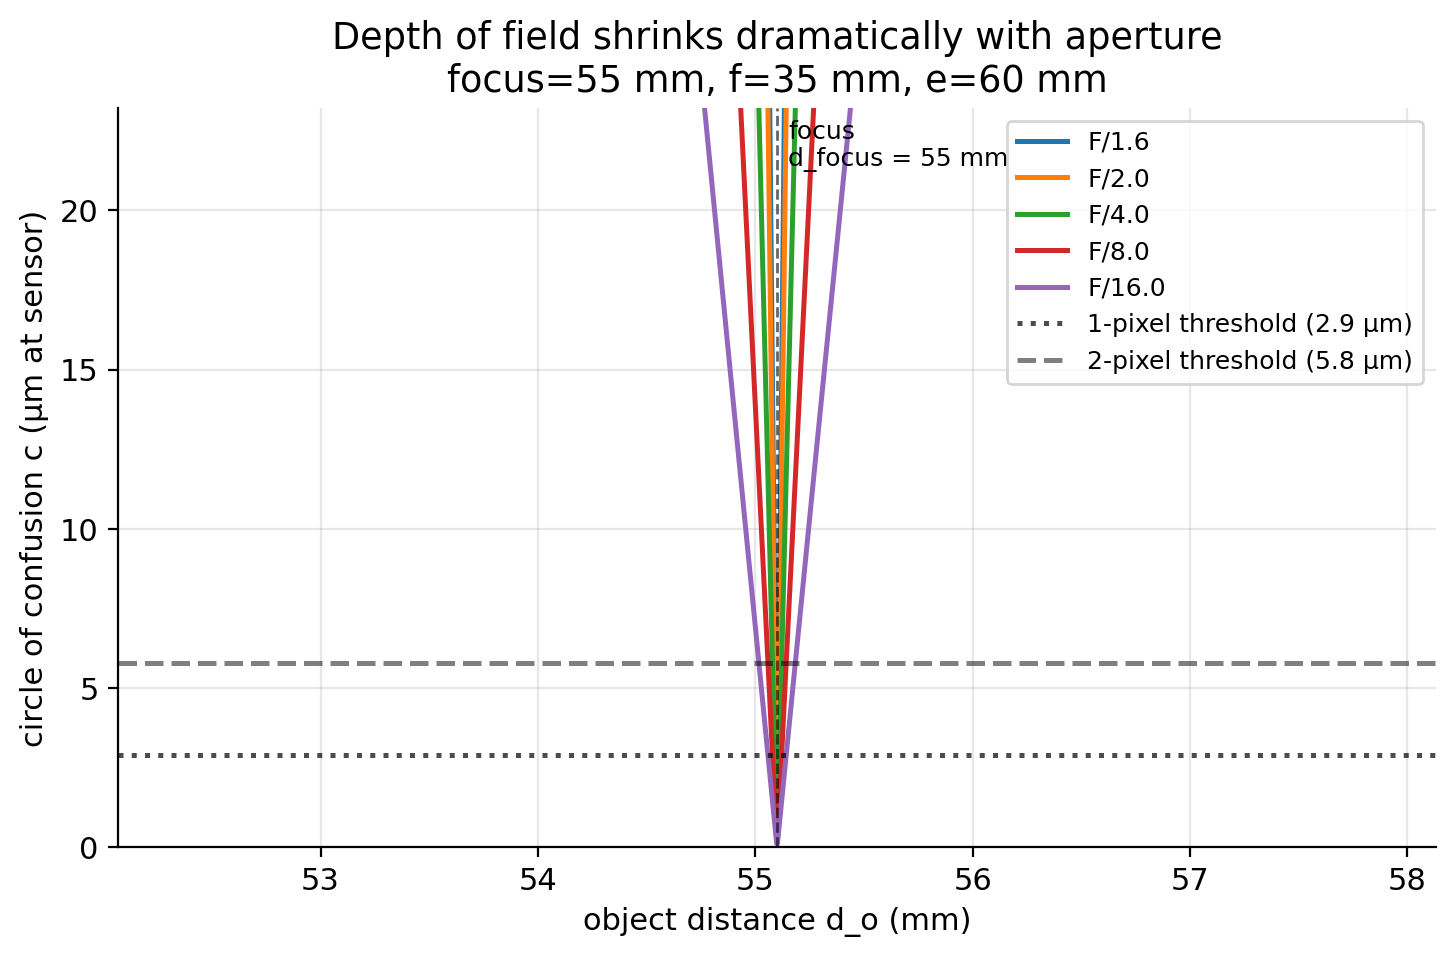
\includegraphics[width=\columnwidth]{04_dof_envelope}
\caption{\textbf{How thick is the in-focus slice at each aperture?} Geometric CoC against object distance for the
engraved iris stops F/1.6, F/2, F/4, F/8 and F/16. Dotted and dashed lines: one and two PAL samples (6.5 and
13.1~\um{} on the sensor). At F/1.6 the CoC stays within one sample over $\pm 9.4$~\um; at F/16 over
$\pm 94$~\um. The curves are geometric; diffraction, not drawn, exceeds one sample beyond about F/4.4
(\secref{sec:dof}).}\label{fig:dof}
\end{figure}

\subsection{Empirical sharpness distribution and frame contamination}\label{sec:empirical}

\code{optics.measure} computes a per-pixel sharpness, $\log(1 + G * (\nabla^2 I)^2)$ with $G$ a $15 \times 15$ Gaussian
kernel, on 120 frames of the case-study clip (every fifth frame), histograms it, and fits a straight line in log--log
coordinates to the density over the band between the 50th and 95th percentiles of its cumulative histogram. The
negative slope $\alpha$ is an empirical descriptor of how fast the density falls past the mode. It is highly
sensitive to the sharp digital and pillarbox edges of \secref{sec:recording} (\tabref{tab:crop}): with no crop
$\alpha = 5.36$, removing the DVR display alone gives 4.57, and removing the pillarbox as well gives 4.88 (fixed
crop) or 4.90 (automatic crop). The two crops that remove both sources agree within 0.4\,\%, whereas the incomplete crops
spread $\alpha$ over 4.57--5.36. Sharp-edged frame contamination must therefore be removed before any sharpness
statistic is interpreted.

\begin{table}
\centering\tabfont
\caption{Fitted slope $\alpha$ of the per-pixel sharpness density for four crops of the case-study clip
(\texttt{scripts/rerun\_paper\_numbers.py}, rows 48--51).}\label{tab:crop}
\begin{tabular}{@{}lr@{}}
\toprule
Crop & $\alpha$ \\
\midrule
none & 5.36 \\
DVR display only (top 55, bottom 120 rows) & 4.57 \\
fixed crop, display and pillarbox ($1800 \times 905$~px) & 4.88 \\
automatic crop, display and pillarbox ($1826 \times 906$~px) & 4.90 \\
\bottomrule
\end{tabular}
\end{table}

We do not read $\alpha$ as a test of the exponent in Eq.~\eqref{eq:sharpness}. That equation describes the sharpness of
an image region as a function of its blur, whereas $\alpha$ describes the distribution over pixels of a smoothed,
log-compressed statistic at unknown and mixed depths. No relation between the two exponents has been derived. Under
the model, a population spread uniformly in depth with $S \propto |\delta|^{-5}$ would give a density of $S$ falling
as $S^{-6/5}$, and a density of $\log S$ falling exponentially rather than as a power law. The closeness of the
cropped $\alpha$ to 5 is therefore not evidence for the model. Directly supported are the crop sensitivity above and
the shape in \figref{fig:measured}: a single mode followed by a shoulder of sharp pixels at a density far below
the peak.

\begin{figure}
\centering
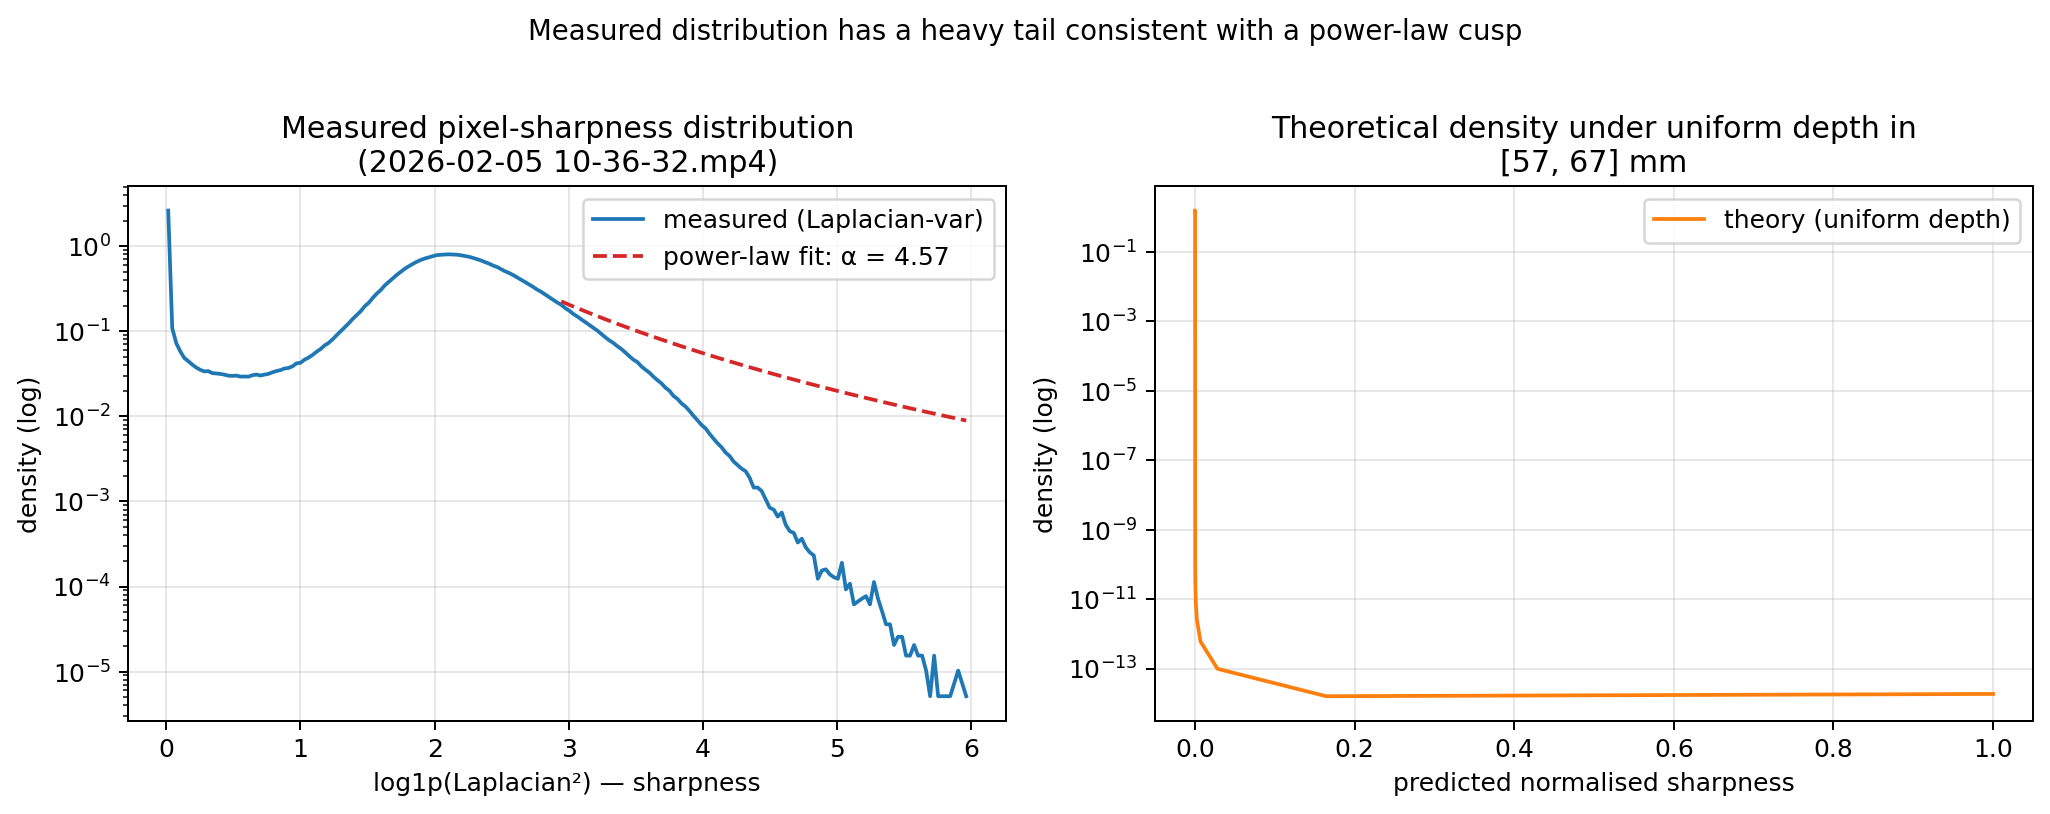
\includegraphics[width=\columnwidth]{08_measured_vs_theory}
\caption{\textbf{What does the measured sharpness distribution look like?} Per-pixel sharpness density of the
case-study clip after the automatic crop (\texttt{optics.measure}). The shaded fit band (50th to 95th percentile of
the cumulative histogram) lies on the decay just right of the mode; the dashed line is the log--log fit over that band,
$\alpha = 4.90$, drawn only where it was fitted. No model density is shown (see text).}\label{fig:measured}
\end{figure}
